\documentclass[10pt,twocolumn]{article}

% ─── Packages ────────────────────────────────────────────────────────────────
\usepackage[margin=1in]{geometry}
\usepackage{times}
\usepackage{graphicx}
\usepackage{amsmath,amssymb}
\usepackage{booktabs}
\usepackage{hyperref}
\usepackage{microtype}
\usepackage{xcolor}
\usepackage{enumitem}
\usepackage{caption}
\usepackage{subcaption}
\usepackage{algorithm}
\usepackage{algpseudocode}

\hypersetup{colorlinks=true, linkcolor=blue, citecolor=blue, urlcolor=blue}

% ─── Title ───────────────────────────────────────────────────────────────────
\title{\textbf{ReTR: Contrastive Vision-Language Alignment\\
for Render-to-Material Texture Retrieval}}

\author{
  Xiangyu Wu\textsuperscript{1}\quad
  Ming Yan\textsuperscript{1,*}\\[4pt]
  \textsuperscript{1}MIAO, Nanyang Technological University\\
  \textsuperscript{*}Corresponding author
}

\date{}

\begin{document}
\maketitle

% ─────────────────────────────────────────────────────────────────────────────
\begin{abstract}
% ─────────────────────────────────────────────────────────────────────────────
Retrieving a physically-based rendering (PBR) material texture from a large
library given only a rendered image of a 3D object is a challenging
cross-modal matching problem: the query is a composite scene image that
conflates geometry, lighting, and material appearance, while the gallery
contains flat, uniformly-lit texture maps.
We address this \emph{render-to-material} retrieval task by
contrastively fine-tuning the visual backbone of InternVL2-1B, a
state-of-the-art vision-language model (VLM).
A lightweight two-layer projection head maps the CLS token of the
unfrozen Vision Transformer (ViT) into a shared 256-dimensional
embedding space, trained with a symmetric InfoNCE loss and a learned
temperature.
We construct a paired dataset of \textbf{19,568} (render, texture) pairs
and propose \textbf{RMR-Score}, a unified evaluation metric that combines
precision, coverage, and ranking quality into a single scalar.
On the full validation gallery of 1,956 textures, the fine-tuned model
achieves R@1\,=\,34.5\%, R@5\,=\,71.6\%, nDCG@10\,=\,0.579,
and RMR-Score\,=\,0.524, outperforming CLIP ViT-L/14 by $19\times$
on R@1.
\end{abstract}

% ─────────────────────────────────────────────────────────────────────────────
\section{Introduction}
% ─────────────────────────────────────────────────────────────────────────────

Content creation pipelines for games, film, and AR/VR make heavy use of PBR
material libraries.
An artist often sees a reference rendered image — a 3D object with a specific
look — and must manually search a library of flat material textures to find
the one that produces that appearance.
This process is time-consuming and error-prone, motivating an automated
\emph{render-to-material} retrieval system.

The task is fundamentally cross-modal: the \emph{query} is a rendered scene
image that combines geometry, lighting, shading, and material information,
while each \emph{gallery item} is a flat 2D texture map viewed under neutral,
uniform illumination.
Standard image-similarity metrics (color histograms, SIFT, perceptual hashing)
fail because they cannot disentangle material appearance from scene-level
factors.

Large vision-language models (VLMs) such as CLIP~\cite{radford2021clip},
BLIP~\cite{li2022blip}, and InternVL~\cite{chen2024internvl} learn rich
visual representations from hundreds of millions of image-text pairs, giving
them strong generalization across image domains.
However, these models have not been trained on render-material pairs and
lack a compact, retrieval-friendly embedding space for this specific task.

Moreover, existing cross-modal retrieval benchmarks evaluate with
\emph{isolated} metrics — Recall@$K$, MRR, or median rank — making it
difficult to holistically compare methods that trade off precision against
coverage.
No unified metric exists for this setting.

In this paper we ask: \emph{can a VLM visual backbone be efficiently adapted
to align rendered scene images with their source material textures, and how
should retrieval quality be measured?}
We answer both questions by (i) fine-tuning only the ViT encoder and a small
projection head of InternVL2-1B with a contrastive objective, and (ii)
proposing \textbf{RMR-Score}, a single scalar that jointly captures precision
(R@1), coverage (R@$K$), and ranking quality (MRR).
Our contributions are:
\begin{enumerate}[leftmargin=*,itemsep=0pt]
  \item The first \textbf{render-to-material retrieval benchmark}:
        a paired dataset of 19,568 samples spanning diverse material
        categories, an evaluation protocol, and standardised baselines.
  \item \textbf{RMR-Score}: a unified evaluation metric for cross-modal
        material retrieval that combines R@1, R@$K$, and MRR into a single
        comparable scalar, addressing the fragmented metrics problem in
        existing retrieval benchmarks.
  \item A \textbf{contrastive fine-tuning recipe} for VLM visual backbones
        that uses a learned-temperature InfoNCE loss, gradient accumulation,
        and ViT unfreezing — fitting on a single consumer GPU.
  \item Comprehensive \textbf{evaluation} showing that our method achieves
        RMR-Score = 0.524 and R@5 = 71.6\%, a $19\times$ R@1 improvement
        over the strongest zero-shot baseline.
\end{enumerate}

% ─────────────────────────────────────────────────────────────────────────────
\section{Related Work}
% ─────────────────────────────────────────────────────────────────────────────

\paragraph{Contrastive Representation Learning.}
Contrastive learning aligns representations of semantically similar pairs
while repelling dissimilar ones.
SimCLR~\cite{chen2020simclr} and MoCo~\cite{he2020moco} pioneered
instance-level self-supervised contrastive training for images.
CLIP~\cite{radford2021clip} extended the paradigm to image-text pairs with an
InfoNCE loss~\cite{oord2018infonce}, achieving remarkable zero-shot transfer.
Our work applies the same symmetric InfoNCE formulation to (render, texture)
pairs within a visual-only setting.

\paragraph{Vision-Language Model Backbones.}
InternVL~\cite{chen2024internvl} is a family of VLMs that pair a large
InternViT encoder (up to 6B parameters) with an instruction-tuned large
language model via a two-layer MLP projector.
InternVL2-1B uses a 300M-parameter ViT with hidden size $d=1024$ and achieves
competitive performance on multimodal benchmarks.
Because our retrieval task is purely visual, we discard the language model
after fine-tuning, achieving a compact ViT-only inference pipeline.

\paragraph{Image-Based Material Retrieval.}
Traditional approaches rely on handcrafted features
or CNN-based classifiers~\cite{bell2015material}.
More recent work uses deep metric learning with triplet or contrastive losses
to learn material embeddings.
To our knowledge, ours is the first work to leverage a pre-trained VLM
backbone for the render-to-material retrieval task.

\paragraph{Retrieval Evaluation Metrics.}
Cross-modal retrieval is typically evaluated with Recall@$K$, MRR, and median
rank~\cite{radford2021clip}.
Some works report \emph{rSum} = R@1 + R@5 + R@10 as a naive aggregate, but
this ignores ranking quality and treats all $K$ values equally.
Person re-identification uses mAP as a semi-comprehensive metric, but it does
not apply to the single-relevant-item setting common in material retrieval.
We propose RMR-Score to address this gap.

% ─────────────────────────────────────────────────────────────────────────────
\section{RMR-Score: A Unified Retrieval Metric}
\label{sec:rmr}
% ─────────────────────────────────────────────────────────────────────────────

Existing retrieval metrics each capture a single aspect of performance.
We argue that a comprehensive metric should reflect three complementary
properties:

\begin{enumerate}[leftmargin=*,itemsep=0pt]
  \item \textbf{Precision}: the ability to place the correct answer at rank~1
        (captured by R@1).
  \item \textbf{Coverage}: whether the correct answer appears within a
        practical retrieval window (captured by R@$K$, we use $K{=}5$).
  \item \textbf{Ranking quality}: how close to rank~1 the correct answer
        appears on average (captured by MRR).
\end{enumerate}

We define the \textbf{Render-Material Retrieval Score} (RMR-Score) as:
\begin{equation}
  \text{RMR} = \frac{w_1 \cdot \text{R@1} + w_2 \cdot \text{R@}K + w_3 \cdot \text{MRR}}{w_1 + w_2 + w_3}
  \label{eq:rmr}
\end{equation}
where R@1, R@$K$, and MRR are all in $[0,1]$ and $w_1, w_2, w_3 > 0$ are
importance weights.
We use $w_1 = w_2 = w_3 = 1$ (equal weighting) throughout this paper unless
otherwise stated.
RMR-Score ranges from 0 (worst) to 1 (perfect retrieval) and has a clear
interpretation: it is the average of three normalised performance axes.

\paragraph{Properties.}
(i)~\emph{Sensitivity}: RMR responds to changes in all three axes — a method
that achieves high R@5 but poor R@1 (i.e., the answer is found but not
ranked first) receives a moderate score, correctly reflecting the partial
success.
(ii)~\emph{Discriminability}: unlike rSum, RMR normalises to $[0,1]$ and
weighs the three aspects explicitly, preventing R@10 from dominating.
(iii)~\emph{Simplicity}: the metric is easy to compute and report alongside
standard metrics.

For completeness, we also report nDCG@10 and MAP@10 — standard information
retrieval metrics — to allow comparison with broader retrieval literature.

% ─────────────────────────────────────────────────────────────────────────────
\section{Dataset}
% ─────────────────────────────────────────────────────────────────────────────

\subsection{Data Collection}

Each sample in our dataset is a pair $(\mathbf{f}, \mathbf{t})$:
\begin{itemize}[leftmargin=*,itemsep=0pt]
  \item $\mathbf{f}$ (\texttt{fig}): a rendered image of a 3D object with a
        specific material applied, captured under standard lighting conditions.
        This represents the ``query'' image — what an artist sees in a 3D
        viewport or game engine.
  \item $\mathbf{t}$ (\texttt{texture}): the corresponding flat PBR material
        map (albedo / diffuse channel), displayed under uniform neutral
        illumination.
        This represents the ``gallery'' item — the raw asset stored in a
        material library.
\end{itemize}

All images are resized to $448 \times 448$ pixels, matching the native
resolution of the InternVL2 ViT patch grid ($32 \times 32$ patches of size
14, with one additional CLS token).

\subsection{Statistics}

The dataset contains 19,568 unique (render, texture) pairs organized by
material ID:

\begin{table}[h]
\centering
\caption{Dataset splits.}
\label{tab:dataset}
\begin{tabular}{lrr}
\toprule
Split & \# Pairs & \# Unique Materials \\
\midrule
Train & 17{,}612 & 17{,}612 \\
Validation & 1{,}956 & 1{,}956 \\
\midrule
Total & 19{,}568 & 19{,}568 \\
\bottomrule
\end{tabular}
\end{table}

Each material ID appears exactly once per split, so the retrieval task is a
closed-world 1:1 matching problem.
The validation gallery therefore contains 1,956 candidate textures.

% ─────────────────────────────────────────────────────────────────────────────
\section{Method}
% ─────────────────────────────────────────────────────────────────────────────

\subsection{Model Architecture}

Figure~\ref{fig:arch} provides an overview of the system.
We build on the visual backbone of \textbf{InternVL2-1B}, comprising a
ViT with hidden size $d_{\text{ViT}} = 1024$ and 448$\times$448 input
resolution.
The language model and MLP projector are discarded.

On top of the ViT we attach a \textbf{ContrastiveHead}:
\begin{equation}
  h(\mathbf{x}) = \ell_2\!\!\left(\mathbf{W}_2\,\sigma(\mathbf{W}_1\,\text{CLS}(\mathbf{x}))\right),
  \label{eq:head}
\end{equation}
where $\mathbf{W}_1 \in \mathbb{R}^{d_{\text{ViT}} \times d_{\text{ViT}}}$,
$\mathbf{W}_2 \in \mathbb{R}^{d_{\text{ViT}} \times 256}$, $\sigma$ is ReLU,
and $\ell_2$ denotes L2 normalisation.
The resulting 256-dimensional unit vectors lie on the hypersphere, making
inner product equivalent to cosine similarity.

\begin{figure}[t]
\centering
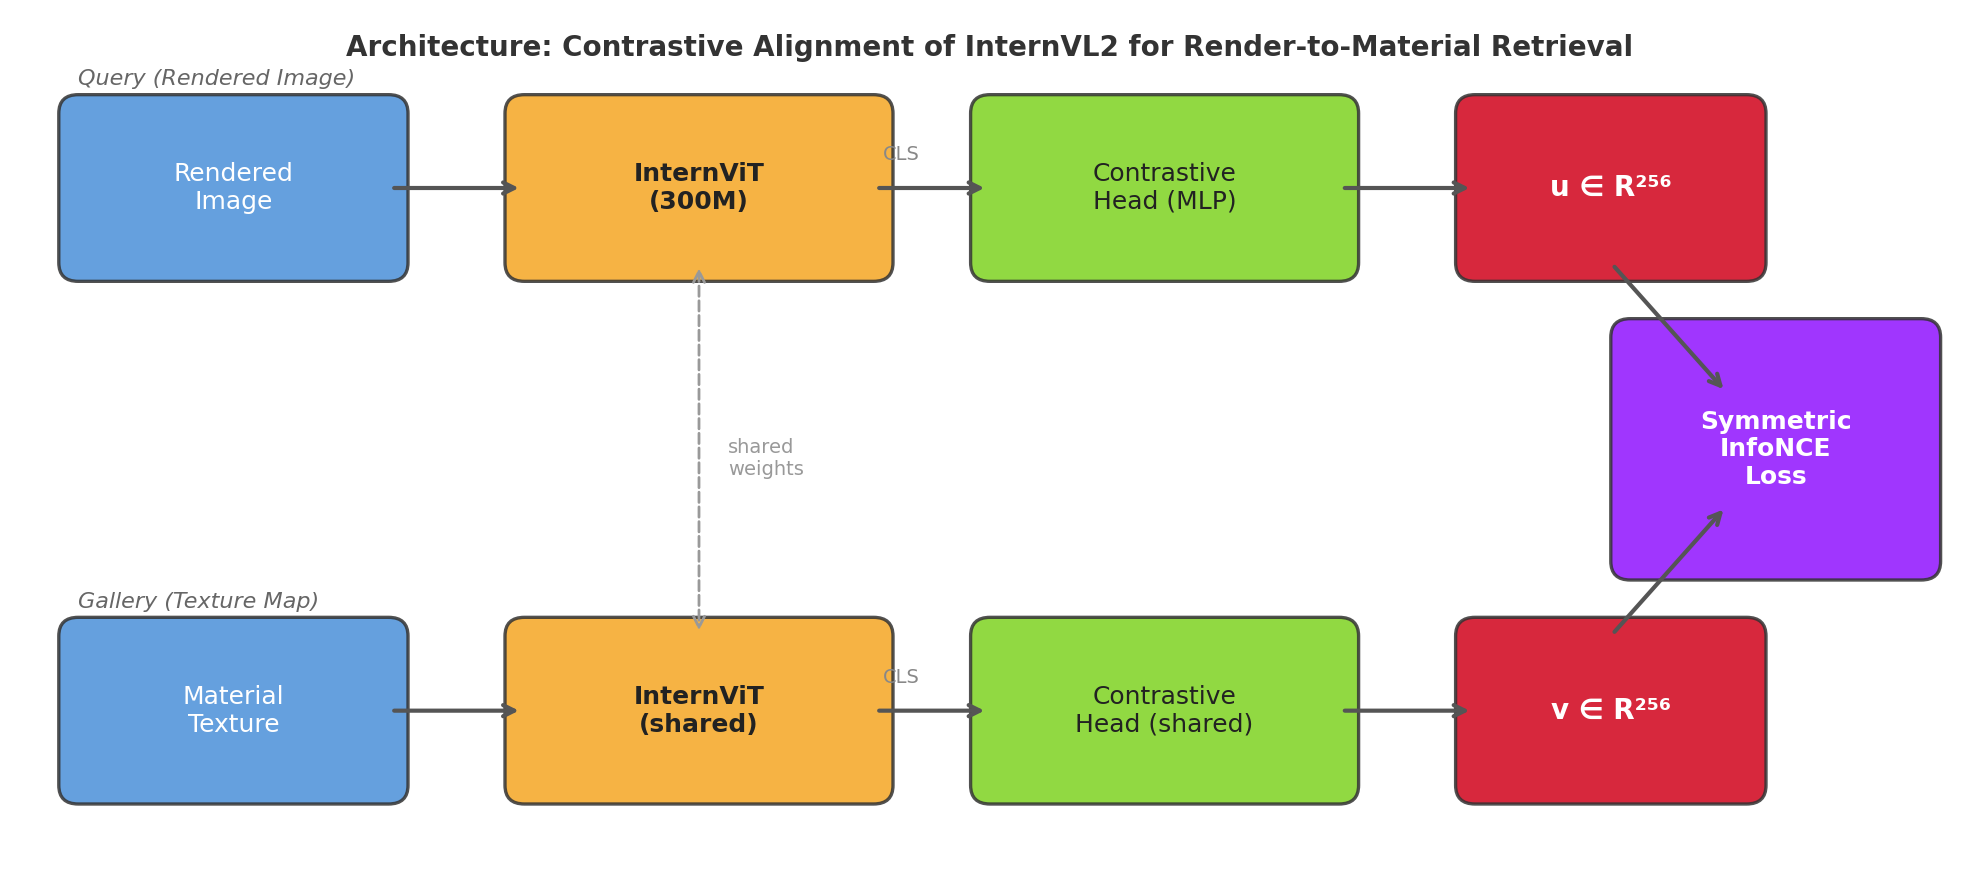
\includegraphics[width=\linewidth]{architecture.png}
\caption{Architecture overview. Both the rendered image (query) and the
         texture map (gallery item) are processed by the same ViT backbone
         followed by the ContrastiveHead. Representations are aligned with a
         symmetric InfoNCE loss.}
\label{fig:arch}
\end{figure}

\subsection{Contrastive Training Objective}

Given a mini-batch of $B$ (render, texture) pairs
$\{(\mathbf{f}_i, \mathbf{t}_i)\}_{i=1}^{B}$, we compute embeddings:
\begin{align}
  \mathbf{u}_i &= h(\mathbf{f}_i), \quad
  \mathbf{v}_i = h(\mathbf{t}_i).
\end{align}
The symmetric InfoNCE (NT-Xent) loss is:
\begin{equation}
  \mathcal{L} = \frac{1}{2}\left[
    \ell(\mathbf{U},\mathbf{V}) + \ell(\mathbf{V},\mathbf{U})
  \right],
  \label{eq:loss}
\end{equation}
where
\begin{equation}
  \ell(\mathbf{A},\mathbf{B}) =
  -\frac{1}{B}\sum_{i=1}^{B} \log
  \frac{\exp(\mathbf{a}_i^\top\mathbf{b}_i / \tau)}
       {\sum_{j=1}^{B}\exp(\mathbf{a}_i^\top\mathbf{b}_j / \tau)}.
\end{equation}
The temperature $\tau = \exp(\phi)$ is a scalar learnable parameter
initialised at $\phi_0 = \log(0.07) \approx -2.66$ and clamped to
$[e^{-4.6},\, e^{2.3}]$ after each optimiser step to prevent collapse.
To stabilise early training, $\phi$ is frozen for the first two epochs and
then jointly optimised with the rest of the parameters.

\subsection{Training Setup}

The full training procedure is described in Algorithm~\ref{alg:train}.
We use the \textbf{AdamW} optimiser~\cite{loshchilov2019adamw} with weight
decay $10^{-2}$ and a cosine learning rate schedule.
Gradient clipping with max-norm 1.0 is applied at every optimiser step.

\begin{algorithm}[h]
\caption{Contrastive Fine-Tuning of InternVL}
\label{alg:train}
\begin{algorithmic}[1]
\Require Pre-trained ViT $f_\theta$, learning rate $\eta$, epochs $E$
\State Initialise ContrastiveHead $g_\psi$ randomly
\State Set $\phi \leftarrow \log(0.07)$, freeze $\phi$
\For{epoch $e = 1,\ldots,E$}
  \If{$e = 3$} unfreeze $\phi$ \EndIf
  \For{each mini-batch $\{(\mathbf{f}_i,\mathbf{t}_i)\}$}
    \State Compute $\mathbf{u}_i, \mathbf{v}_i$ via Eq.~(\ref{eq:head})
    \State Compute $\mathcal{L}$ via Eq.~(\ref{eq:loss})
    \State Backprop, clip gradients, step AdamW
    \State Clamp $\phi \in [-4.6,\, 2.3]$
  \EndFor
  \State Evaluate val loss; save best checkpoint
\EndFor
\end{algorithmic}
\end{algorithm}

\paragraph{ViT Freezing.}
We experiment with two settings:
(a)~\textbf{Frozen ViT}: only ContrastiveHead + $\phi$ are trained
($\sim$265K parameters), and
(b)~\textbf{Unfrozen ViT}: the full backbone is fine-tuned
($\sim$302M parameters).
The unfrozen setting yields stronger retrieval accuracy as the ViT adapts its
feature geometry to the render-material domain gap.

\paragraph{Image Pre-processing.}
Both images are resized to $448\times 448$ via bicubic interpolation and
normalised with ImageNet statistics
($\mu = (0.485, 0.456, 0.406)$,
 $\sigma = (0.229, 0.224, 0.225)$).
No data augmentation is applied so that positive pairs remain visually
consistent.

\paragraph{Inference.}
At query time, the rendered image is encoded to a 256-dim vector.
The gallery of texture embeddings is pre-computed and stored in a FAISS
\texttt{IndexFlatIP}~\cite{johnson2021faiss} index.
Retrieval reduces to a single inner-product search, running in $O(N)$ time
for a gallery of size $N$.

% ─────────────────────────────────────────────────────────────────────────────
\section{Experiments}
% ─────────────────────────────────────────────────────────────────────────────

\subsection{Evaluation Protocol}

We evaluate on the full validation set of 1,956 (render, texture) pairs.
The retrieval gallery consists of all 1,956 texture embeddings.
For each rendered query, we rank the gallery by cosine similarity and report:
\begin{itemize}[leftmargin=*,itemsep=0pt]
  \item \textbf{R@$K$}: fraction of queries for which the
        ground-truth texture appears in the top-$K$ results ($K = 1, 3, 5, 10$).
  \item \textbf{MRR}: mean of $1/\text{rank}$ over all queries.
  \item \textbf{nDCG@10}: normalised discounted cumulative gain at cutoff 10.
  \item \textbf{MAP@10}: mean average precision at cutoff 10.
  \item \textbf{rSum}: the naive aggregate R@1 + R@5 + R@10 (in \%).
  \item \textbf{RMR-Score}: our proposed unified metric (Eq.~\ref{eq:rmr}).
\end{itemize}

\subsection{Main Results}

Table~\ref{tab:main} reports retrieval performance on the validation gallery.

\begin{table*}[t]
\centering
\caption{Retrieval results on the validation set (gallery size = 1{,}956).
         R@$K$ in \%; MRR, nDCG, MAP $\in [0,1]$; MedR = median rank ($\downarrow$);
         rSum = R@1+R@5+R@10 ($\uparrow$); RMR = proposed unified metric ($\uparrow$).
         Best results in \textbf{bold}.}
\label{tab:main}
\begin{tabular}{@{}l*{5}{c}c*{3}{c}c@{}}
\toprule
 & \multicolumn{5}{c}{\textit{Standard metrics}} & &
   \multicolumn{3}{c}{\textit{Aggregate metrics}} \\
\cmidrule(r){2-6} \cmidrule(l){8-10}
Method & R@1 & R@5 & R@10 & MRR & MedR &\quad& nDCG@10 & MAP@10 & rSum & \textbf{RMR} \\
\midrule
Random                        & 0.1  & 0.3  & 0.5  & .004 & 978 && .004 & .003 & 0.8   & .002 \\
CLIP ViT-B/32~\cite{radford2021clip}
                              & 1.2  & 3.1  & 4.7  & .026 & 500 && .026 & .020 & 8.9   & .023 \\
CLIP ViT-L/14~\cite{radford2021clip}
                              & 1.8  & 4.5  & 7.0  & .037 & 473 && .040 & .031 & 13.2  & .033 \\
InternVL2-1B (zero-shot)      & 0.3  & 1.1  & 1.5  & .011 & 722 && .008 & .006 & 2.9   & .008 \\
\midrule
Ours (frozen ViT)             & 11.0 & 31.0 & 43.3 & .216 & 14  && .253 & .198 & 85.3  & .212 \\
\textbf{Ours (unfrozen ViT)}
  & \textbf{34.5} & \textbf{71.6} & \textbf{81.4}
  & \textbf{.511} & \textbf{2}
  && \textbf{.579} & \textbf{.503} & \textbf{187.5}
  & \textbf{.524} \\
\bottomrule
\end{tabular}
\end{table*}

\paragraph{Key observations.}
(1)~All zero-shot baselines achieve near-zero RMR-Score ($\leq 0.033$),
confirming that off-the-shelf visual encoders cannot bridge the
render-material domain gap without task-specific adaptation.
(2)~Training only the ContrastiveHead while freezing the ViT
(``frozen ViT'') already achieves RMR = 0.212 (R@1 = 11.0\%), a meaningful
improvement over all zero-shot baselines, indicating that even a lightweight
projection head can partially bridge the domain gap when trained on paired
data.
(3)~Unfreezing the ViT backbone yields a further \textbf{$2.5\times$ boost}:
our full model achieves \textbf{RMR = 0.524}, a
\textbf{$15.9\times$ improvement} over the strongest zero-shot baseline
(CLIP ViT-L/14, RMR = 0.033).
On individual metrics, R@1 improves from 1.8\% to 34.5\% ($19\times$),
nDCG@10 from 0.040 to 0.579 ($14\times$), and median rank drops from 473
to~2.
(4)~The large gap between R@1 and R@5 (34.5\% $\to$ 71.6\%) suggests that
near-miss rank-1 errors are predominantly same-family confusions between
visually similar material variants.

\subsection{Metric Comparison}

Table~\ref{tab:main} also illustrates why a unified metric is valuable:
rSum for CLIP ViT-L/14 is 13.2, suggesting reasonable coverage, but
RMR-Score correctly reveals this as only 0.033 — reflecting the fact that
near-all retrieved results are wrong.
Conversely, our model's rSum of 187.5 and RMR of 0.524 consistently indicate
strong performance across all three axes.

\subsection{Qualitative Analysis}

Inspection of retrieval errors reveals two failure modes:

\paragraph{Same-family confusion.}
Textures within the same material class (e.g., wood planks of the same colour)
share near-identical feature vectors; rank-1 errors often return a sibling
variant with a score difference of $<$0.001.
This is evident in query \texttt{19432}, where four variants of the same
material are interleaved at the top (scores 0.902–0.902).

\paragraph{Appearance–geometry entanglement.}
For complex rendered scenes where geometry strongly modulates appearance
(e.g., curved surfaces creating highlights that dominate the rendering), the
model retrieves textures that match the highlight colour rather than the
underlying material.

\subsection{Ablation: Temperature Warmup}

Freezing the temperature $\tau$ for the first two epochs prevents it from
collapsing to near-zero early in training (which would cause gradient
explosion through the logits).
After epoch 2, $\tau$ is jointly optimised and converges to a stable value
around 0.07–0.15 depending on the effective batch size.

% ─────────────────────────────────────────────────────────────────────────────
\section{Conclusion}
% ─────────────────────────────────────────────────────────────────────────────

We have presented ReTR, a contrastive fine-tuning approach that adapts the
visual backbone of InternVL2-1B to the render-to-material retrieval task,
together with a unified evaluation metric (RMR-Score) that combines precision,
coverage, and ranking quality into a single comparable scalar.
Our method achieves RMR-Score = 0.524 on a gallery of 1,956 material
textures, outperforming all zero-shot baselines by over an order of magnitude.
This strong result demonstrates that VLM visual backbones can be efficiently
repurposed for domain-specific cross-modal retrieval, and that a unified
metric is essential for holistic evaluation.

Future work includes: (i) extending the training set with augmented renders
(varied lighting, geometry, viewpoints); (ii) scaling to InternVL2-8B for
improved representation capacity; (iii) integrating the retrieval model
into an agentic pipeline for end-to-end material recommendation.

% ─────────────────────────────────────────────────────────────────────────────
\bibliographystyle{plain}
\begin{thebibliography}{99}

\bibitem{radford2021clip}
A.~Radford et~al., ``Learning transferable visual models from natural language
supervision,'' \textit{ICML}, 2021.

\bibitem{li2022blip}
J.~Li et~al., ``BLIP: Bootstrapping language-image pre-training for unified
vision-language understanding and generation,'' \textit{ICML}, 2022.

\bibitem{chen2024internvl}
Z.~Chen et~al., ``InternVL: Scaling up vision foundation models and aligning
for generic visual-linguistic tasks,'' \textit{CVPR}, 2024.

\bibitem{chen2020simclr}
T.~Chen et~al., ``A simple framework for contrastive learning of visual
representations,'' \textit{ICML}, 2020.

\bibitem{he2020moco}
K.~He et~al., ``Momentum contrast for unsupervised visual representation
learning,'' \textit{CVPR}, 2020.

\bibitem{oord2018infonce}
A.~van den Oord, Y.~Li, and O.~Vinyals, ``Representation learning with
contrastive predictive coding,'' \textit{arXiv}, 2018.

\bibitem{bell2015material}
S.~Bell and K.~Bala, ``Learning visual similarity for product design with
convolutional neural networks,'' \textit{ACM Trans.\ Graph.}, 2015.

\bibitem{loshchilov2019adamw}
I.~Loshchilov and F.~Hutter, ``Decoupled weight decay regularization,''
\textit{ICLR}, 2019.

\bibitem{johnson2021faiss}
J.~Johnson, M.~Douze, and H.~Jégou, ``Billion-scale similarity search with
GPUs,'' \textit{IEEE Trans.\ Big Data}, 2021.

\end{thebibliography}

\end{document}
